\documentclass[UTF8]{ctexart}
\usepackage{graphicx} % Required for inserting images
\usepackage{subfigure}
\title{电路基础实验}
\author{BrightMoon}
\date{May 2024}

\begin{document}

\maketitle

\section{三极管驱动电磁铁}
用LabVIEW控制DAQ的输出电压,从而控制三极管的基极,从而控制三极管的通断,进而控制电磁铁。参考图\ref{DAQ控制电磁铁(代码)}\ref{DAQ控制电磁铁(正视)}\ref{DAQ控制电磁铁(俯视)}。

\begin{figure}
\centering  %图片全局居中
\subfigure[DAQ控制电磁铁(正视)]{
\label{DAQ控制电磁铁(正视)}
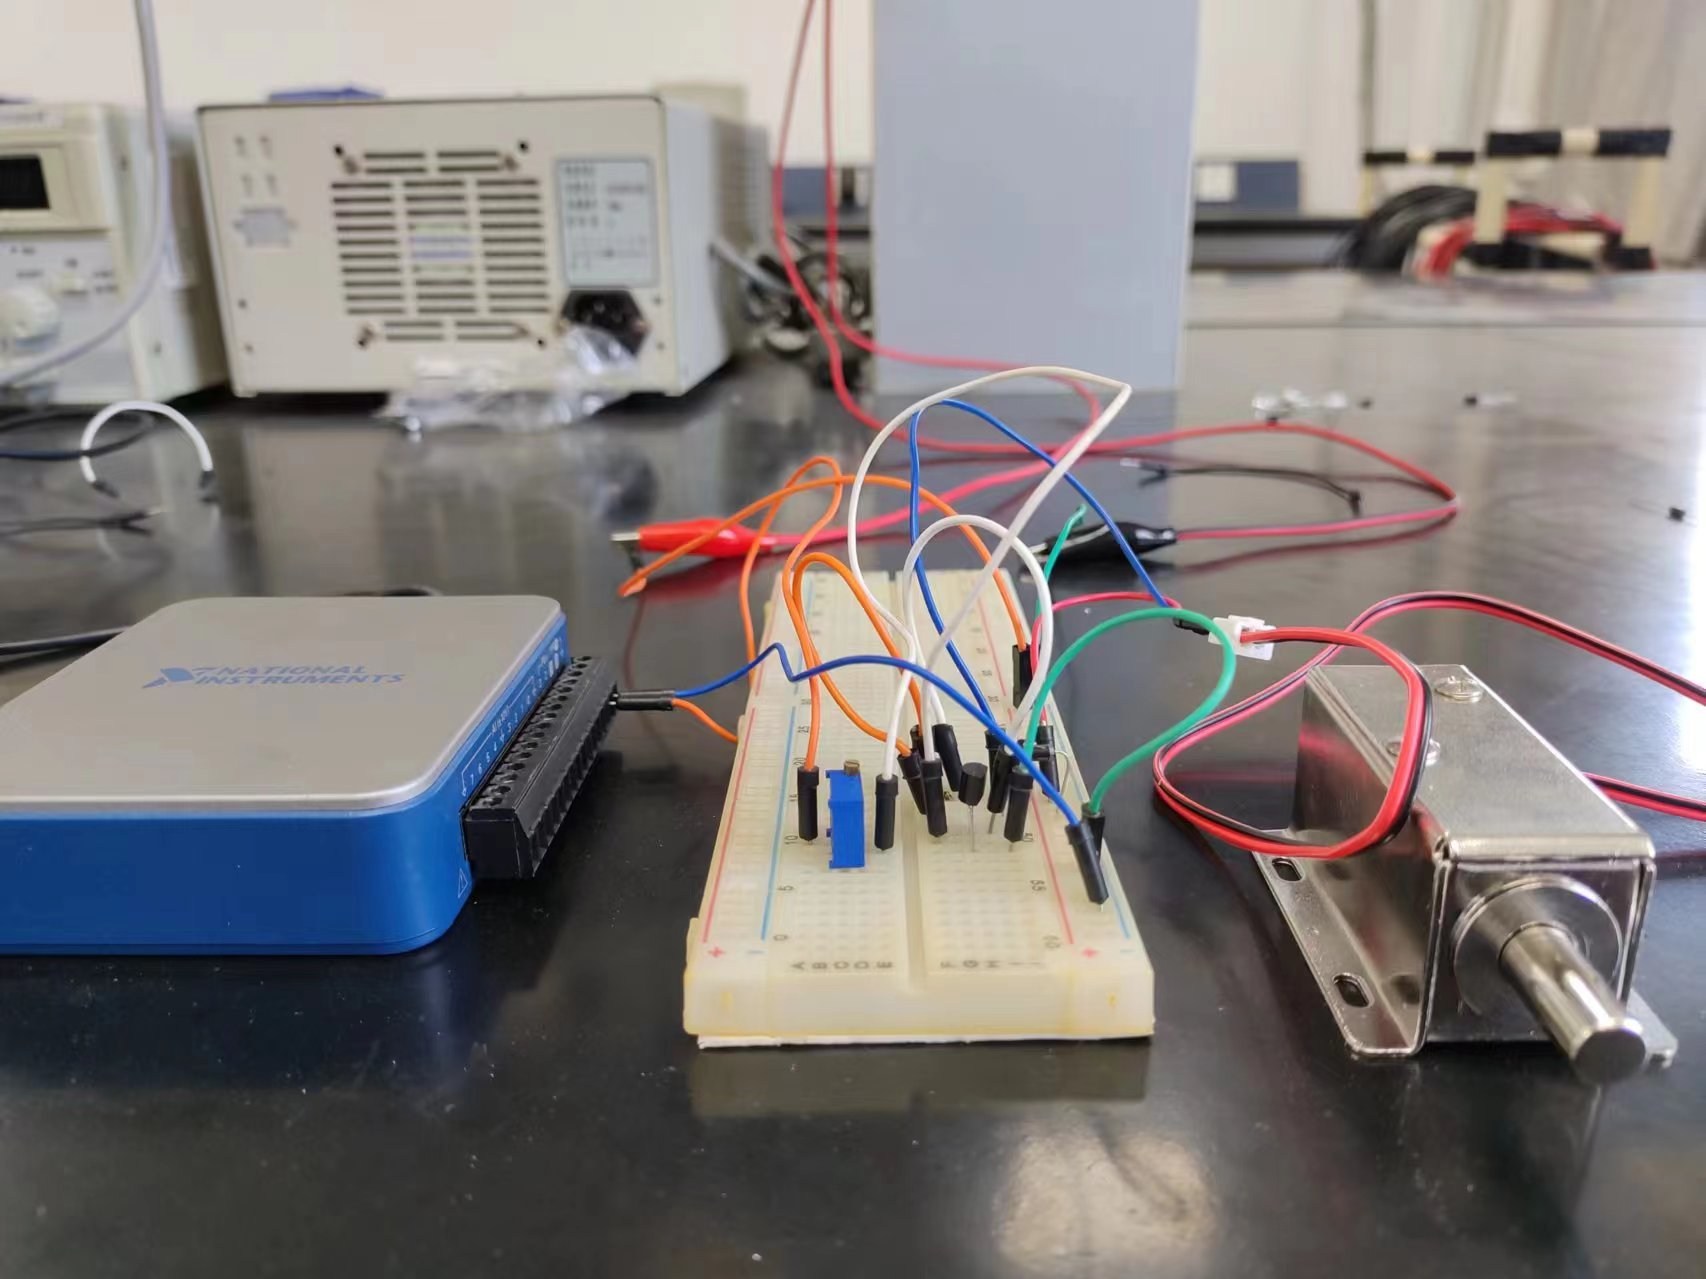
\includegraphics[width=3.2cm,height = 3cm]{electromagnet1.jpg}}
\subfigure[DAQ控制电磁铁(俯视)]{
\label{DAQ控制电磁铁(俯视)}
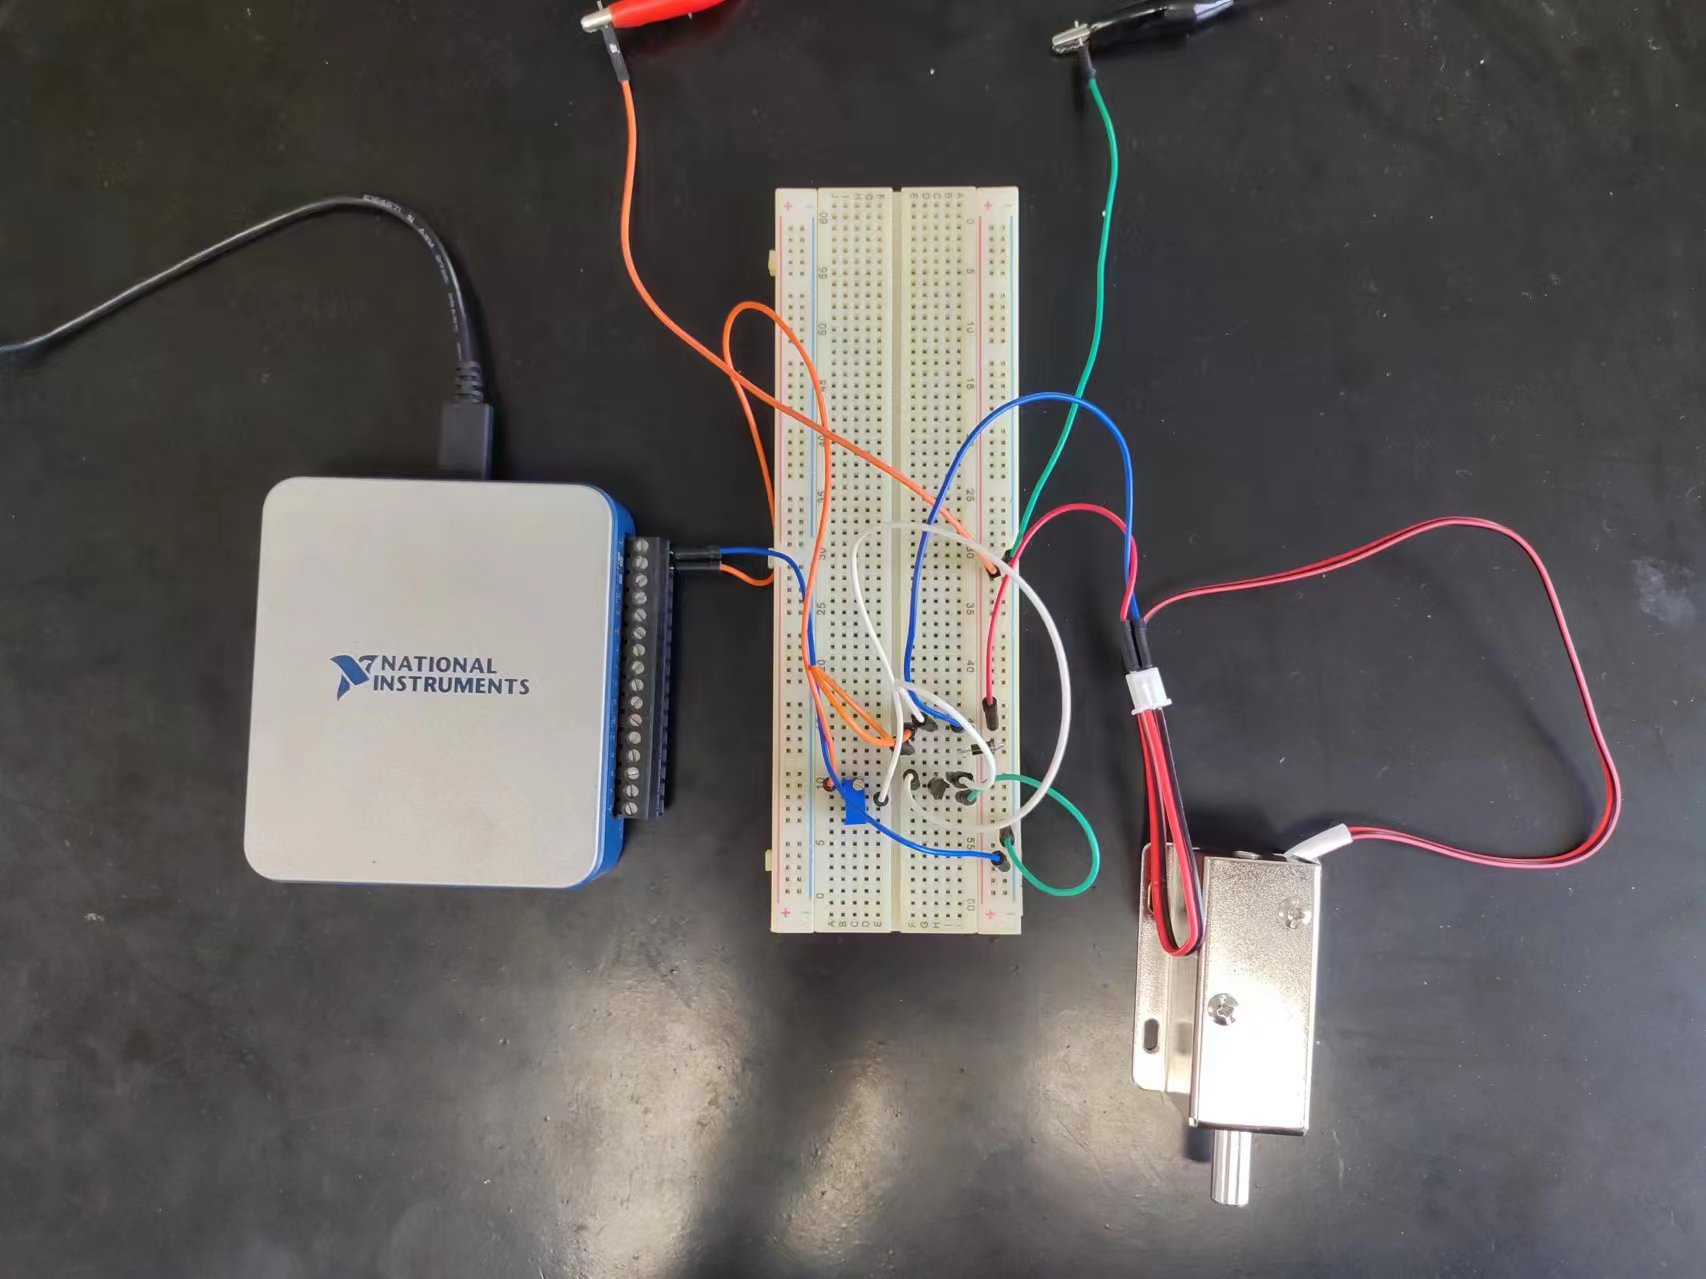
\includegraphics[width=3.2cm,height = 3cm]{electromagnet2.jpg}}
\subfigure[DAQ控制电磁铁(代码)]{
\label{DAQ控制电磁铁(代码)}
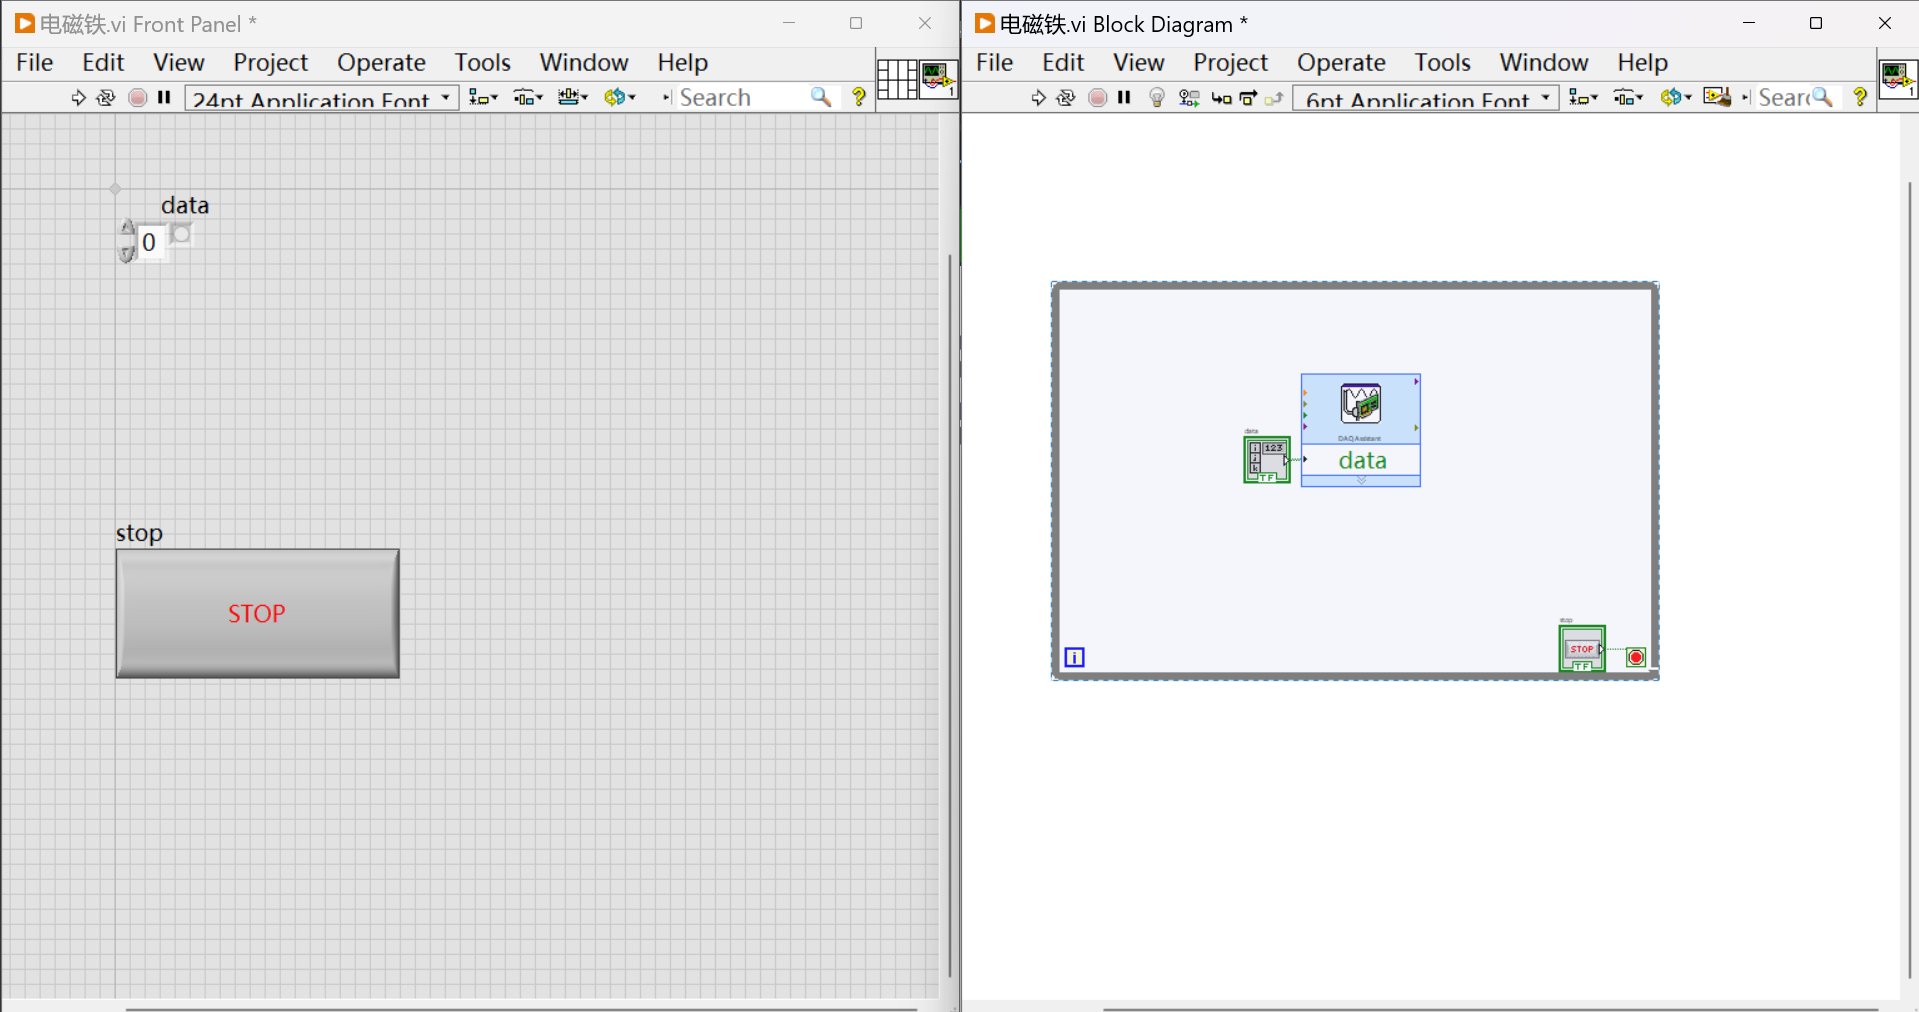
\includegraphics[width=3.2cm,height = 3cm]{code_of_ele.png}}
\caption{DAQ控制电磁铁}
\end{figure}

\section{运算放大器}
\subsection{原理的理解}
老师说的$V_+=V_-$,我觉得可以从两方面理解。
\begin{enumerate}
\item $V_{out}=A(V_+-V_-),\quad A>>1;V_{out} \in [-15,+15]$ 所以,$V_+\approx V_-$ 。
\item $V_-$增大,$V_{out}$减小;$V_-$减小,$V_{out}$增大(\textbf{负输入端与输出端的反向变化})。利用这一点,把负输入端和输出端并联在同一个电阻两端,再通过设计电路(\textbf{电压波动改变电流,电流大小调节电压}),使之形成一个负反馈调节的系统。由于运算放大器极其敏感(上式中A很大),\textbf{所以反馈调节很强,使得$V_+\approx V_-$ 可以很稳定地保持。}(在图\ref{Inverting op-amp}和\ref{Non-inverting op-amp}中做了标识)

\end{enumerate}
在$V_+\approx V_-$ 的基础上,计算后续公式就很简单了。
\subsection{单纯的运算放大器}
如图\ref{Operational Amplifier}所示,给一个运算放大器的正负输入端提供不同电压,检测输出电压。结果见表\ref{pure op}。

\subsection{Non-inverting Amplifier}
按照图\ref{Non-inverting op-amp}搭建电路,更换不同阻值电阻,测量结果见表\ref{Non-inverting Amplifier}。
\subsection{Inverting Amplifier}
按照图\ref{Inverting op-amp}搭建电路,更换不同阻值电阻,测量结果见表\ref{inverting Amplifier}。
\begin{table}
    \centering
    \begin{tabular}{|c|c|c|c|} \hline 
         组别&  $V_+$(v)&  $V_-$(v)& $V_{out}$(v)\\ \hline 
         1&  0&  +15& -13.64\\ \hline 
         2&  0&  -15& +14.46\\ \hline 
         3&  0&  -9.75& +13.67\\ \hline
    \end{tabular}
    \caption{单纯的运算放大器实验}
    \label{pure op}
\end{table}


\begin{table}
    \centering
    \begin{tabular}{|c|c|c|c|l|l|c|} \hline 
         组别&  $R_1(\Omega)$&  $R_2(\Omega)$&  理论增益值$\frac{V_{out}}{V_{in}}=\frac{R_1+R_2}{R_1}$&   $V_{in}$(v)&$V_{out}$(v)&实际增益值\\ \hline 
         1&  61.5k&  12.1k&  1.20&   12.0&14.2&1.18\\ \hline 
         2&  74.2&  12.1k&  164&   0.1&14.1&141\\ \hline 
         3&  12.1k&  74.2&  1.00&   15.0&14.6&0.97\\ \hline
    \end{tabular}
    \caption{Non-inverting Amplifier}
    \label{Non-inverting Amplifier}
\end{table}
\begin{table}
    \centering
    \begin{tabular}{|c|c|c|c|l|l|c|} \hline 
         组别&  $R_1(\Omega)$&  $R_2(\Omega)$&  理论增益值$\frac{V_{out}}{V_{in}}=-\frac{R_2}{R_1}$&   $V_{in}$(v)&$V_{out}$(v)&实际增益值\\ \hline 
         1&  74.2&  61.5k&  828&   0.01&-14.3&-1430\\ \hline 
         2&  12.1k&  61.5k&  5.06&   0.1&-0.509&-5.09\\ \hline 
         3&  1.00k&  61.5k&  61.5&   0.01&-0.617&-61.7\\ \hline
    \end{tabular}
    \caption{Inverting Amplifier}
    \label{inverting Amplifier}
\end{table}

\begin{figure}
\centering  %图片全局居中
\subfigure[Operational Amplifier]{
\label{Operational Amplifier}
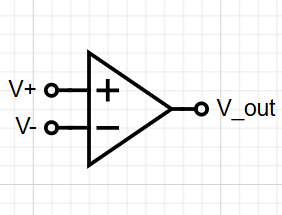
\includegraphics[width=3.2cm,height = 3cm]{pure op.png}}
\subfigure[Inverting op-amp]{
\label{Inverting op-amp}
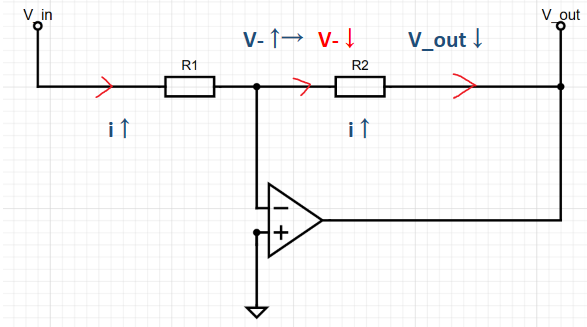
\includegraphics[width=3.2cm,height = 3cm]{inverting.png}}
\subfigure[Non-inverting op-amp]{
\label{Non-inverting op-amp}
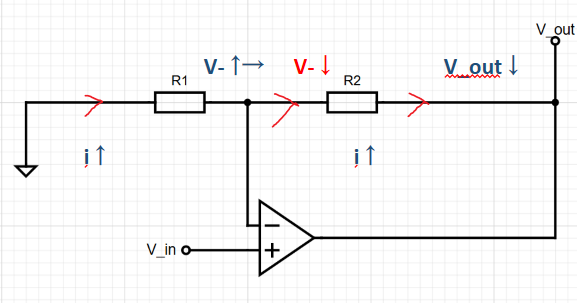
\includegraphics[width=3.2cm,height = 3cm]{noninverting.png}}
\caption{Operational Amplifier:在后两个图中,我对反馈调节的机制做了标识,蓝色代表电压波动,红色是在波动之后反馈调节的结果。}
\end{figure}

\section{发光二极管}
\subsection{LED I-U曲线}
我希望通过DAQ测量LED的电流,这样更方便分析处理。但是,DAQ作为一个电流表有很大的内阻。于是,采用伏阻法(类似灵敏电流计改装电流表)。但是,实验室电阻普遍过大。于是采用滑动变阻器,调节到小电阻位置,测量其阻值,作为小定值电阻使用。设计电路和代码如图\ref{电路图}和\ref{数据处理代码}所示。操作步骤如下:
\begin{enumerate}
    \item 调节电源电压,从2.5V开始,每10秒种,增加0.1V(DAQ每十秒钟采集一次)。到5.3V截止。
    \item 根据所得数据,把定值电阻的电压转化成LED的电流。这一步骤在后期用Python 完成。然后绘制曲线。

\end{enumerate}

根据所得结果,我认为LED电压在4.2V以前,I-U曲线比较符合理论曲线。但是4.2V再往上,电流的增长速率放缓,这意味着阻值相对比较大了。实验的时候,我的手在LED上方可以感觉到比较热,我担心烧坏LED,于是没有再往上加电压了。
\begin{figure}
\centering  %图片全局居中
\subfigure[电路图]{
\label{电路图}
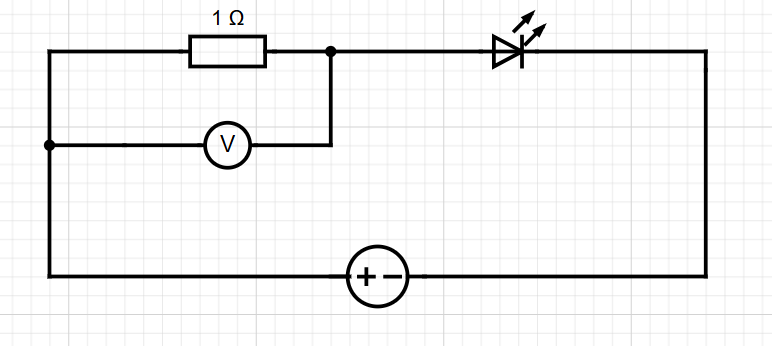
\includegraphics[width=5cm,height = 3cm]{measure current.png}}
\subfigure[相关代码]{
\label{数据处理代码}
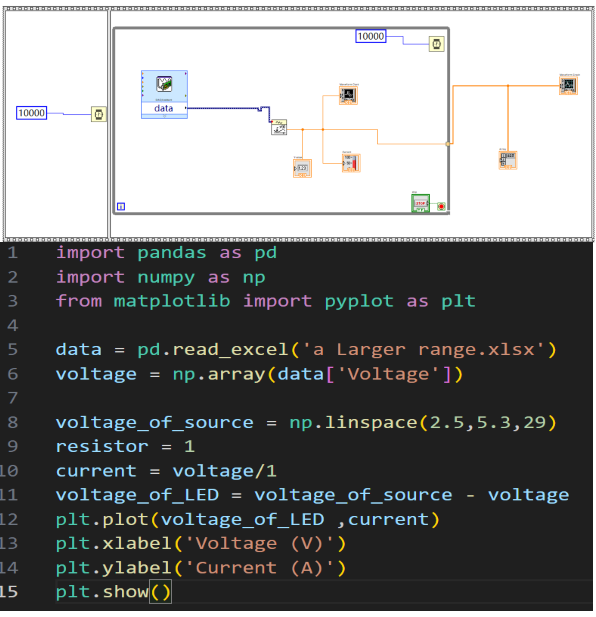
\includegraphics[width=5cm,height = 3cm]{coding.png}}
\subfigure[I-U 曲线]{
\label{I-U曲线}
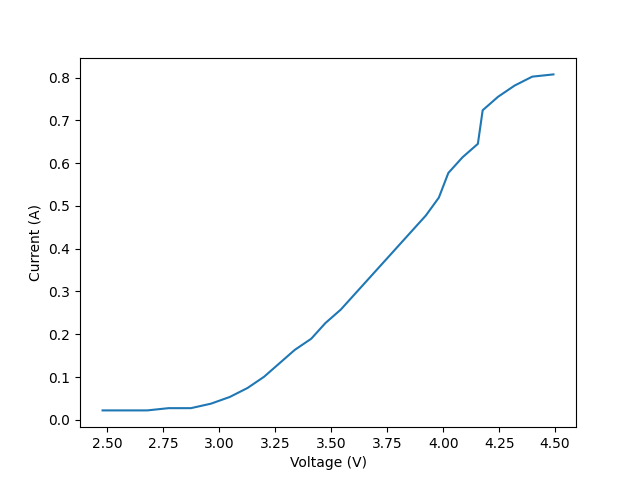
\includegraphics[width=5cm,height = 3cm]{I_U.png}}
\subfigure[I-U 曲线(LabVIEW 采集画面,可以动态监测)]{
\label{I-U曲线 LabVIEW}
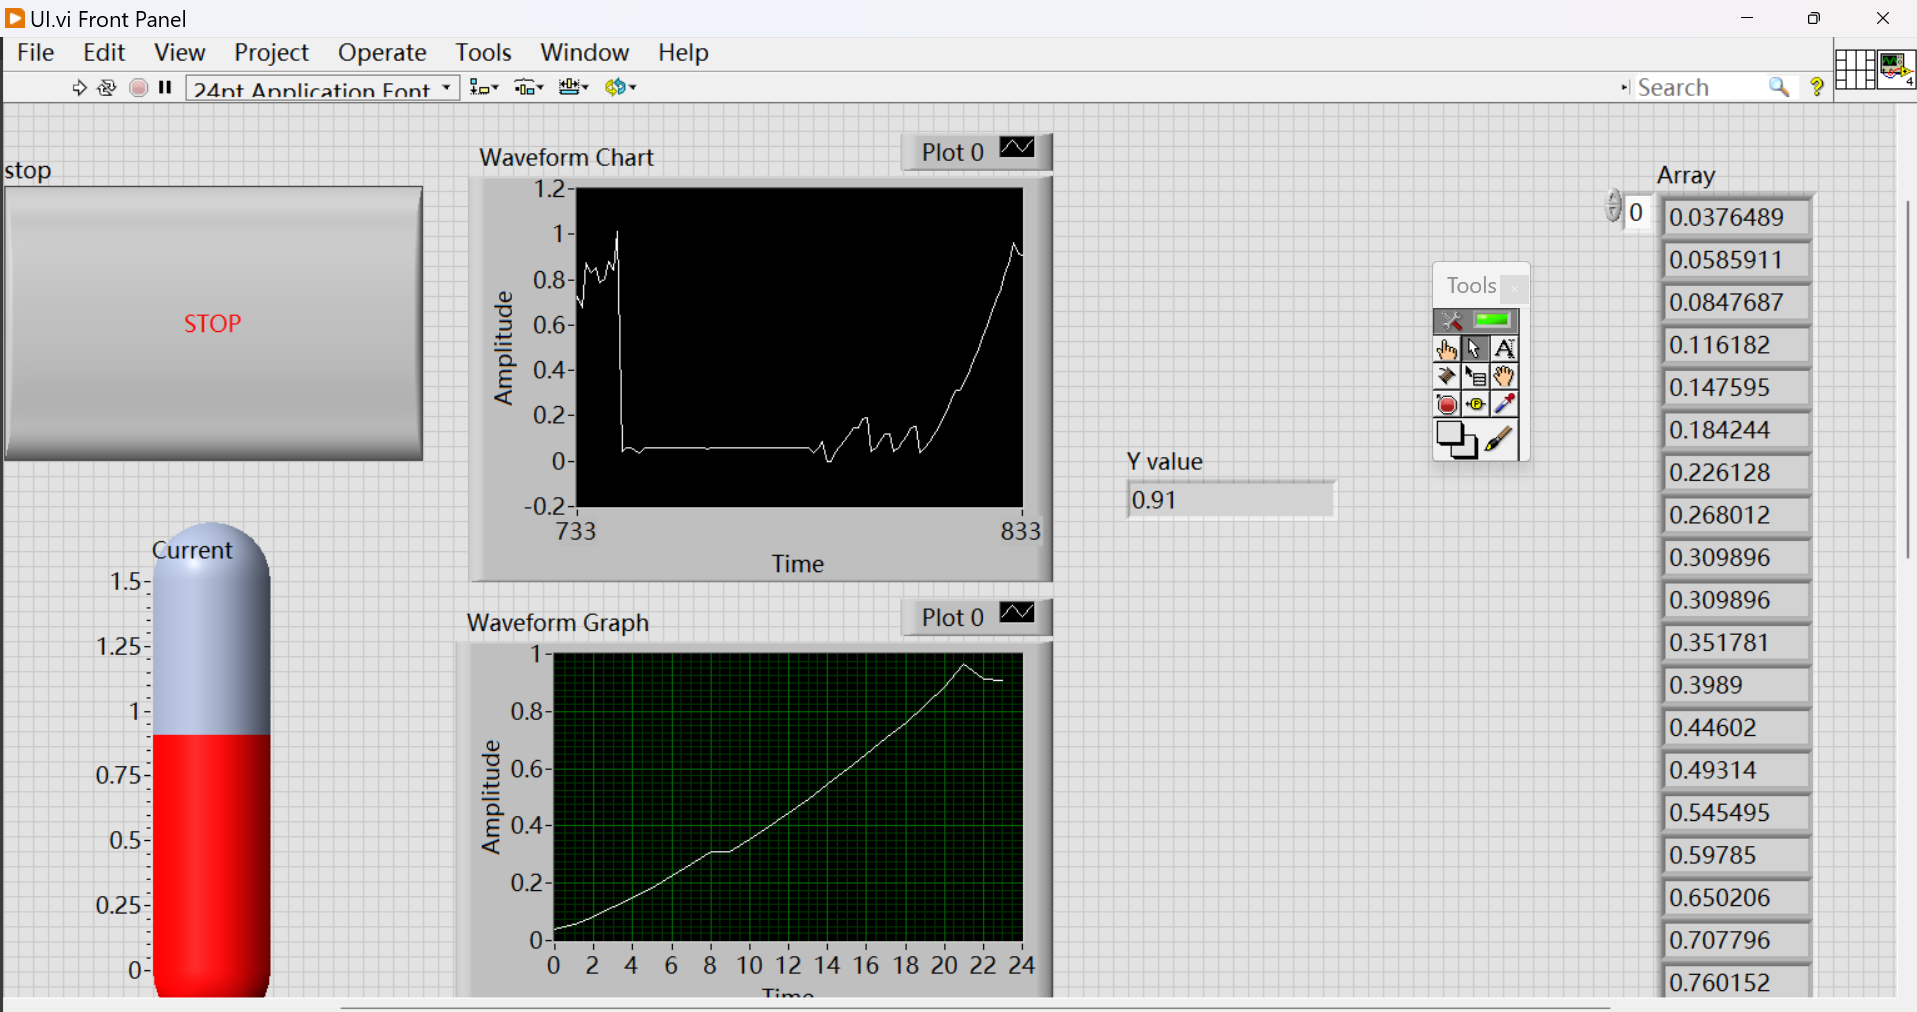
\includegraphics[width=5cm,height = 3cm]{1.png}}
\caption{LED I-U 曲线}
\end{figure}
\subsection{搭建LED控制电路}
搭建电路。调节滑动变阻器,控制LED电流,明暗变化与预期一致。

加上交流电后,可以观察到LED闪烁。改变交流电频率,发现闪烁频率与交流电频率变化趋势一致。

\begin{figure}
\centering  %图片全局居中
\subfigure[电路]{
\label{电路}
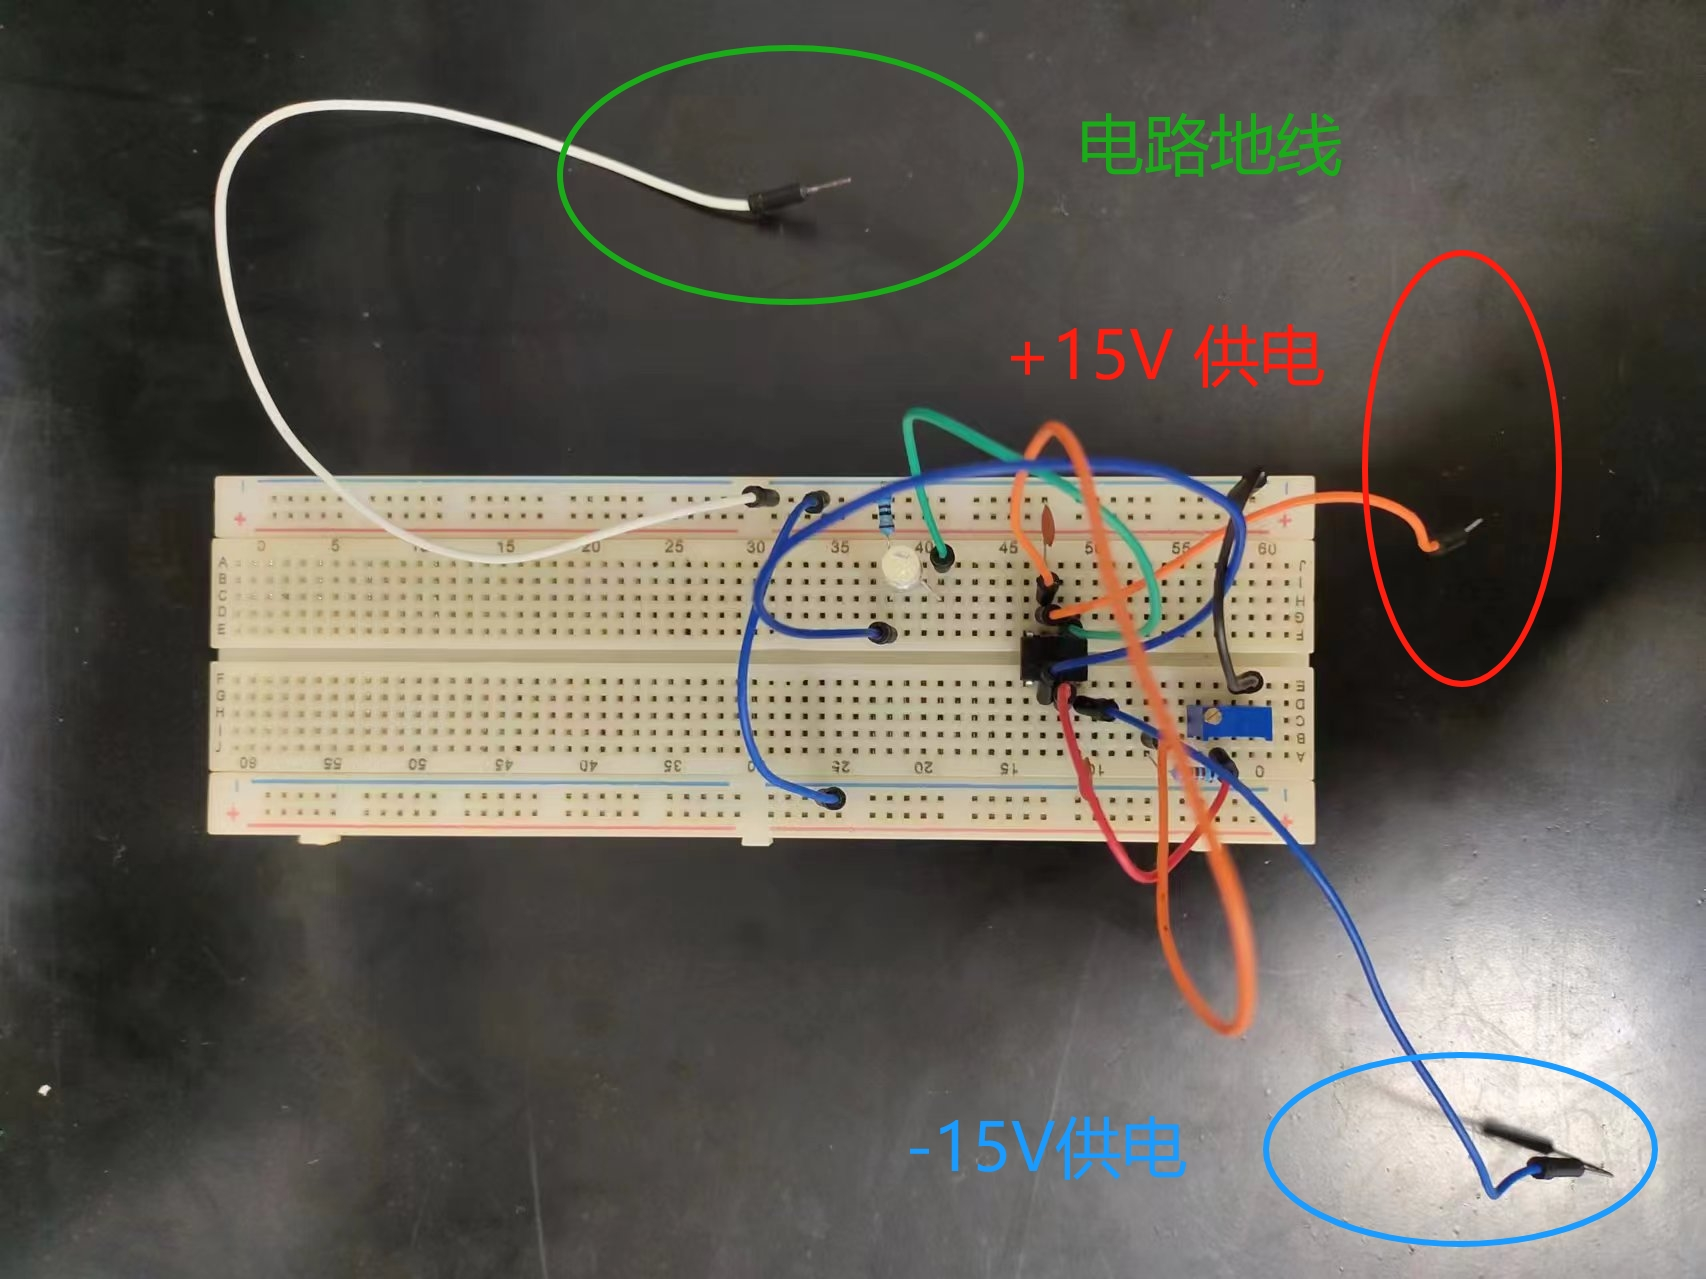
\includegraphics[width=5cm,height = 3cm]{LED.jpg}}
\subfigure[电路工作效果图]{
\label{电路工作效果}
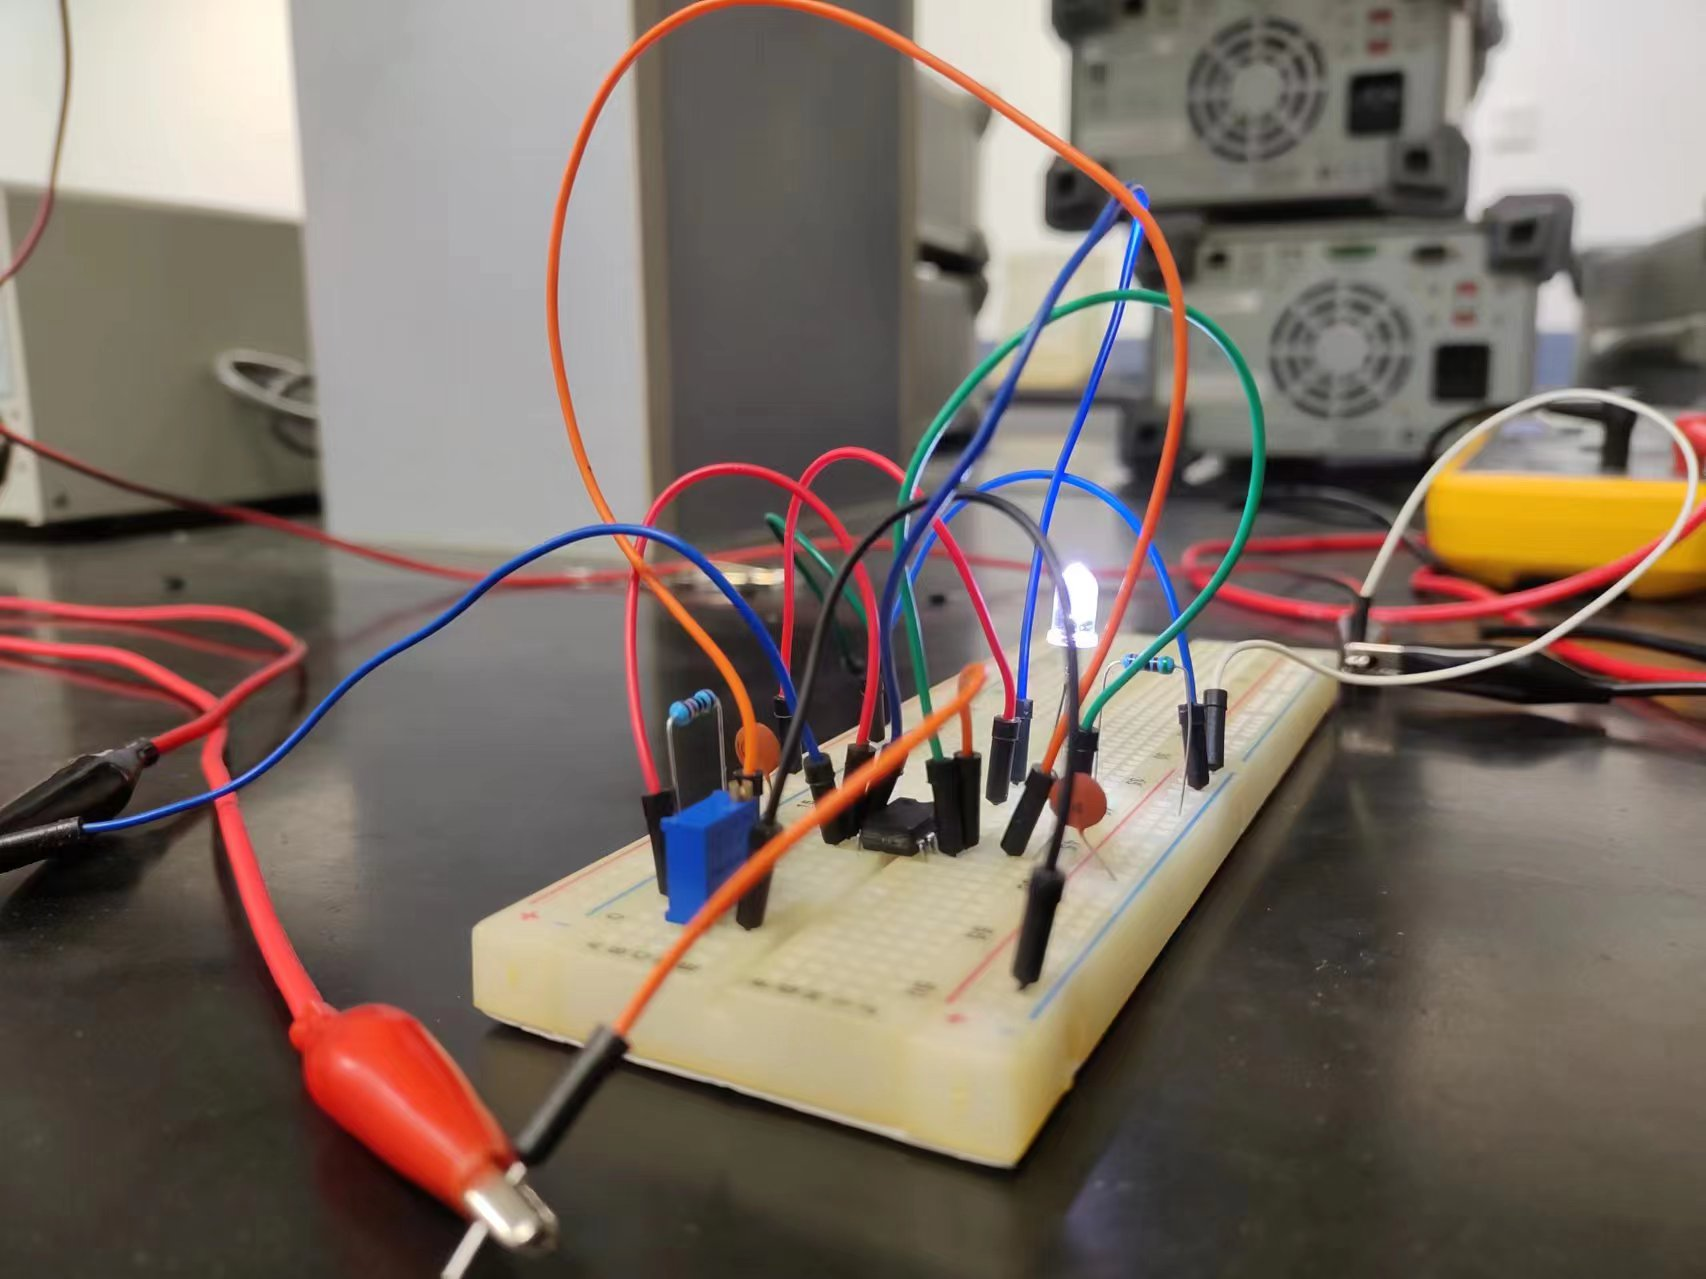
\includegraphics[width=5cm,height = 3cm]{workingLED.jpg}}
\caption{LED控制电路}
\end{figure}


\end{document}
